\documentclass{article}	

\usepackage[utf8]{inputenc}
\usepackage{amsmath}
\usepackage[german]{babel}
\usepackage{amssymb}
\usepackage{amsxtra}
\usepackage[dvips]{epsfig,psfrag}
\usepackage{listings}
\usepackage{url}
\usepackage[numbers]{natbib}

\bibliographystyle{plainnat}

\newcommand{\refchapter}[1]{Kapitel~\ref{#1}}
\newcommand{\refsec}[1]{Sektion~\ref{#1}}
\newcommand{\refeqn}[1]{Gleichung~(\ref{#1})}
\newcommand{\reffig}[1]{Abbildung~\ref{#1}}

\title{
{\bf \scriptsize RHEINISCH-WESTF\"ALISCHE TECHNISCHE HOCHSCHULE AACHEN \\
LuFG Informatik 12 (Prof. Dr. rer. nat. Uwe Naumann)}
\vspace{.5cm} \\

\epsfig{file=figures/STCE_Logo_WWW.eps,width=.7\textwidth}
\vspace{1cm} \\
{\bf \Large Korrelation und Regressionsanalyse} \\
{\large Proposal} 
}

\author{vorgelegt von Patrick Neidig (Matr.-Nr. ??????)\\
	und Marius Grysla (Matr.-Nr. 274047)}

\begin{document}

\lstloadlanguages{[ISO]C++}
\lstset{basicstyle=\small, numbers=left, numberstyle=\footnotesize,
  stepnumber=1, numbersep=5pt, breaklines=true, escapeinside={/*@}{@*/}}


\pagestyle{headings}

\maketitle

%\newpage
%\tableofcontents % Brauchen wir für das Proposal ein Inhaltsverzeichnis?

\newpage

\section{Einleitung}
Wer behandelt welches Thema?

\subsection{Motivation}

\section{Korrelation}

\section{Regressionsanalyse}

Der zweite große Teil der Arbeit wird sich mit der Regressionsanalyse beschäftigen.
Die NAG-Bibliothek bietet dazu zahlreiche Funktionen, von verschiedenen Regressionsarten bis hin zu Hilfen für die Bewertung und Validierung von Regressionsmodellen.
Daher wird sich dieser Teil wieder in zwei Teile 

\subsection{Regressionsmodelle}
Welche Regressionsarten werden von der Bibliothek unterstützt? $\Rightarrow$ Referenzen auf Grundlagen zu den Regressionsarten\\
Welche davon werden in der Arbeit behandelt? $\Rightarrow$ Einfache, Multivariante, robuste


\section{Leistungsanalyse}

Die zwei wichtigsten Eigenschaften von mathematischen Funktionen sind Korrektheit und Ressourcenverbrauch.
Eine gute Funktion sollte daher für alle möglichen Parameter den mathematisch korrekten Wert berechnen und dies zudem mit möglichst wenig Ressourcen, wie Speicher oder Prozessor-Laufzeit.
Da die NAG C-Bibliothek bereits seit 1990 entwickelt wird\cite{Wikipedia:nag} und zudem alle Methoden vor der Veröffentlichung auf Korrektheit geprüft werden\cite{NAG2011}, ist nicht davon auszugehen, dass Fehler vorhanden sind.
Daher wird in der Ausarbeitung nur die Leistung behandelt.

Dazu sollen zwei Algorithmen der Bibliothek auf ihren Ressourcenverbrauch untersucht werden: Der Bravais-Pearson Korrelationskoeffizient und die multiple lineare Regression.
Für beide werden Laufzeit und Speicherverbrauch unter Benutzung von verschiedenen Parametern mit ansteigender Komplexität untersucht.
Damit alle Berechnungen vergleichbar sind, werden sie auf dem RWTH Cluster ausgeführt.

\section{Zeitplan}

Der Zeitplan für die Seminararbeit und die verschiedenen Präsentationen richtet sich hauptsächlich nach den vorgegebenen Terminen.
Eine Übersicht über die Arbeitsschritte wird in Abbildung \ref{fig:Zeitplan} gezeigt.
\begin{figure}[t]
 %TODO: Bild verkleinern?
 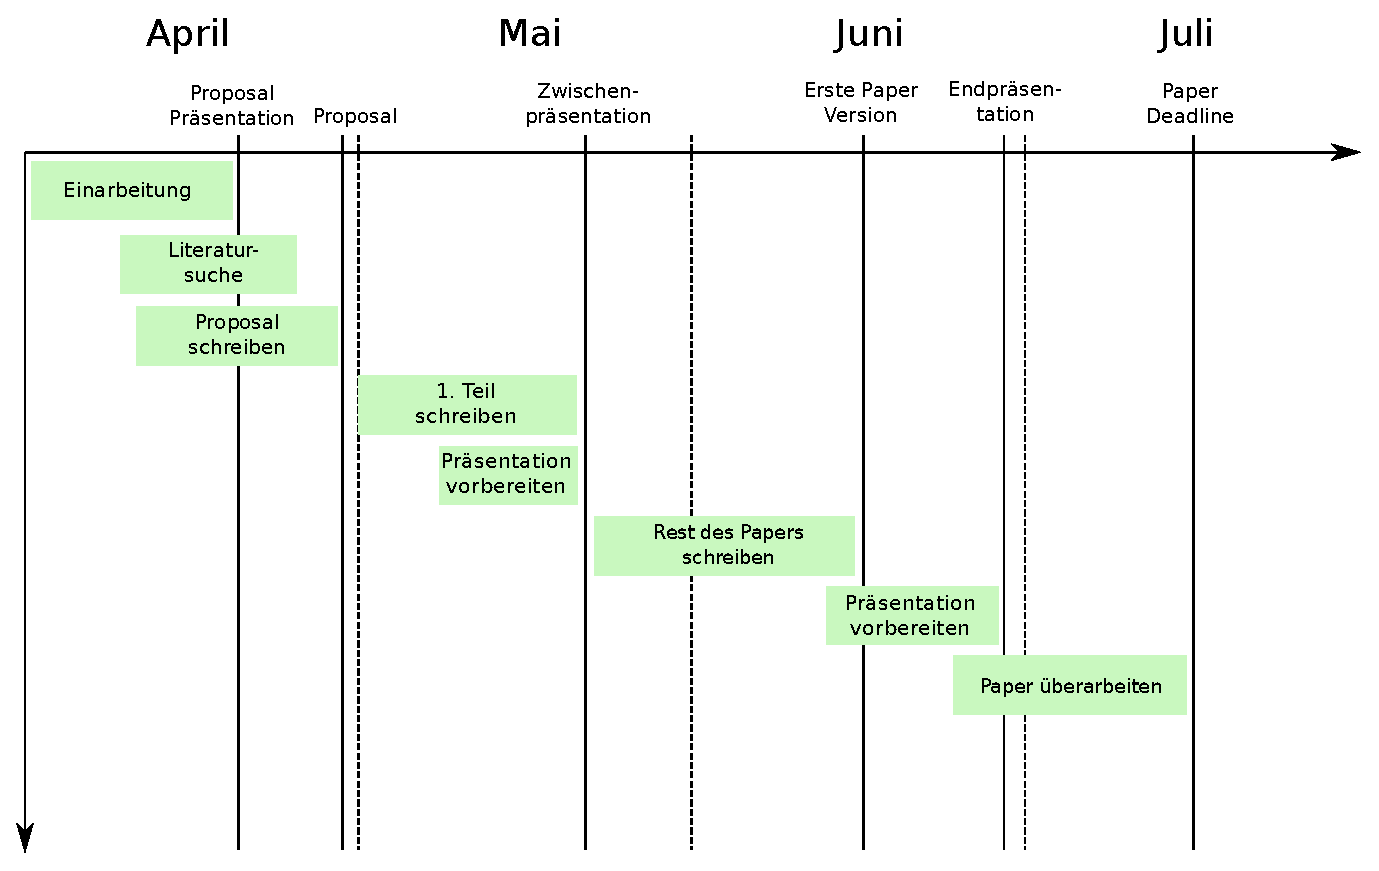
\includegraphics[width=\linewidth]{./figures/Workplan-adj.eps}
 \caption{Der geplante Arbeitsverlauf mit Abgabezeitpunkten.}
 \label{fig:Zeitplan}
\end{figure}
Auf der x-Achse ist dabei der Zeitverlauf und auf der y-Achse die Arbeitsschritte abgebildet.

Der erste Teil besteht aus der Einarbeitung in die statistischen Grundlagen, sowie in die verfügbaren Funktionen der Bibliothek.
Darauf folgt eine Literatursuche, deren Fokus auf auf den mathematischen Funktionen hinter den NAG-Funktionen liegt.
Nach der Abgabe dieses Proposals werden wir mit dem Schreiben des ersten Teils der Arbeit beginnen. 
%TODO: @Patrick: Ist das richtig so?
Dieser soll neben der Einleitung aus der Behandlung von jeweils einer Funktion für Korrelation und Regression bestehen, welche dann auch in der Zwischenpräsentation vorgestellt werden.
Bis zum ersten Abgabetermin Mitte Juni wird die Ausarbeitung dann noch um weitere Algorithmen und eine Laufzeitanalyse erweitert.
%TODO: Was wird noch in der Hauptpräsentation vorgestellt?
In der letzten Präsentation werden die Ergebnisse der Analyse präsentiert und außerdem wird die Benutzung der Bibliothek anhand eines größeren Beispiels demonstriert.
Zuletzt soll die Ausarbeitung noch einmal überarbeitet und Fehler korrigiert werden.

Da wir da Thema nur zu zweit bearbeiten ist kein wirklicher Notfallplan vorgesehen. 
Falls das Seminar von einem Teammitglied abgebrochen wird, werden die Grundlagen vom jeweils Anderen übernommen, der dafür seinen Themenbereich entsprechend kürzer behandelt.

%TODO: Bibliothek einbinden
\bibliography{report}


\end{document}

